% Scientific Reports submission (Springer Nature sn-jnl, sn-nature)
\documentclass[pdflatex,sn-nature,lineno]{sn-jnl}

\usepackage{graphicx}
\usepackage{amsmath,amssymb,amsfonts}
\usepackage{textcomp}
\usepackage{xcolor}
\usepackage{booktabs}
\usepackage{algorithm}
\usepackage{algpseudocode}
\usepackage{microtype}
\usepackage[htt]{hyphenat}
\usepackage{placeins}
\usepackage{needspace}
\hyphenation{Tiny-Llama Re-verse-Adap-tive com-mu-ni-ca-tion in-struc-tion-fol-low-ing}
% Allow more floats near their citations (class defaults starve the queue under [!t]).
\setcounter{topnumber}{3}
\setcounter{bottomnumber}{2}
\setcounter{totalnumber}{4}
\renewcommand{\topfraction}{0.9}
\renewcommand{\bottomfraction}{0.7}
\renewcommand{\textfraction}{0.07}
\renewcommand{\floatpagefraction}{0.7}
\renewcommand{\dbltopfraction}{0.9}
\renewcommand{\dblfloatpagefraction}{0.7}
% Force black, borderless links (class email macro otherwise forces blue)
\hypersetup{hidelinks}
% Break DOIs/URLs at punctuation only (hyperref already loaded by the class)
\makeatletter
\def\UrlBreaks{\do\.\do\/\do\-\do\_\do\~\do\=\do\#\do\:\do\;\do\,\do\?\do\&\do\+\do\%}%
% Class \ps@headings already uses a zero-height head box at \vspace*{-48pt} but
% leaves the head text empty (\hfill\relax\hfill) for production; filling
% \leftmark / author here is required for a self-contained preprint PDF.
% \markboth alone does not surface heads because the class never prints the marks.
\def\ps@headings{%
  \let\@mkboth\markboth
  \def\@oddfoot{\hfill\thepage\hfill}%
  \let\@evenfoot\@oddfoot
  \def\@evenhead{%
    \vbox to 0pt{\vspace*{-48pt}%
      \hbox to \hsize{\footnotesize\itshape Jerry Adams Franklin\hfill}}\par
    \hspace*{-\textwidth}\hbox to \hsize{\hfill}}%
  \def\@oddhead{%
    \vbox to 0pt{\vspace*{-48pt}%
      \hbox to \hsize{\hfill\footnotesize\itshape\leftmark}}\par
    \hspace*{-\textwidth}\hbox to \hsize{\hfill}}%
}
% Opening page: same centered folio as \ps@headings, no running head.
% (Class \ps@titlepage uses a different footer box, which shifted the page-1 number.)
\def\ps@firstpage{%
  \let\@mkboth\markboth
  \def\@oddfoot{\hfill\thepage\hfill}%
  \let\@evenfoot\@oddfoot
  \def\@oddhead{}\def\@evenhead{}}
% Shadows class \email (blue text + trailing semicolon). Revert first if the
% publisher's build complains about the redefinition.
\def\email#1{\global\advance\emailcnt by 1\relax
  \if@corauemail
    \g@addto@macro\corrauthemail{%
      \setcounter{footnote}{0}%
      \textcolor{black}{#1}%
    }%
  \else
    \g@addto@macro\authemail{%
      \setcounter{footnote}{0}%
      \textcolor{black}{#1}%
    }%
  \fi}
\makeatother
\providecommand{\doiurl}[1]{\url{https://doi.org/#1}}

\begin{document}

\title[Measured Comm.\ Frontier for Federated LoRA]{A Measured Communication-Quality Frontier for Federated LoRA Fine-Tuning with Adaptive Phase-Switching}

\author*{\fnm{Jerry Adams} \sur{Franklin}}\email{franklin.je@northeastern.edu}
\affil*{\orgname{Independent Researcher}, \orgaddress{\city{Fairport}, \state{NY}, \postcode{14450}, \country{USA}}}

\abstract{Federated fine-tuning of large language models with low-rank adaptation (LoRA) reduces the number of trainable parameters, but communication remains the dominant cost, and protocols are usually compared by parameter-count ratios rather than by measured bytes. This paper measures per-round upload and download bytes for five federated LoRA protocols, three of them from prior work, and places them on a single communication-quality frontier scored by held-out instruction-following loss. The frontier has a knee. ReverseAdaptive, which learns both LoRA factors before freezing one once the relative improvement in training loss falls below a dimensionless threshold, sits at that knee: it cuts measured round-trip communication by 40.5\% relative to FLoRA at a held-out loss cost of 0.0063, and beats FFA-LoRA, which freezes that factor at initialization, by 0.0182 in held-out loss, more than twenty times the largest per-method seed standard deviation. The same threshold carries to LLaMA-3.2-3B without retuning, where it saves 30.0\%.}

\keywords{federated learning, low-rank adaptation, communication efficiency, large language models, measurement}

\maketitle
\pagestyle{headings}
\thispagestyle{firstpage}

\section{Introduction}
\label{sec:intro}

Federated learning enables model training across distributed clients without sharing raw data, making it attractive for privacy-sensitive applications of large language models (LLMs) \cite{kairouz2021advances}. Fine-tuning with low-rank adaptation (LoRA) \cite{hu2022lora} substantially reduces the number of trainable parameters per client, but federated LoRA aggregation still transmits nontrivial bytes per round. Because adapters cross the network in every round, cumulative communication often determines whether a protocol is deployable where uplink bandwidth is scarce or metered.

LoRA \cite{hu2022lora} parameterizes a weight update as a low-rank product $BA$, so each client trains and transmits two small matrices rather than a full update. Existing federated LoRA methods differ in what they aggregate and when. FedIT \cite{zhang2024federatedgpt} applies FedAvg \cite{mcmahan2017communication} to $A$ and $B$ separately, paying full bidirectional cost per round; because the optimal global update is the product $BA$ rather than a product of separately averaged factors, this introduces aggregation error that grows with client heterogeneity. FFA-LoRA \cite{sun2024ffalora} removes the mismatch by freezing $A$ at initialization so that clients train and transmit only $B$ from the first round, a theoretical 50\% upload saving; the original work also motivates the frozen-$A$ design in terms of differential privacy. FLoRA \cite{wang2024flora} preserves product-space semantics by stacking client modules and compressing them with singular value decomposition (SVD), at full bidirectional cost, and is the full-state baseline in the experiments below. FedSA-LoRA \cite{guo2025fedsalora} makes the opposite choice to FFA-LoRA and shares only $A$; under the byte accounting of Methods, that transmits 64\% of the full TinyLlama state rather than 36\%. FlexLoRA \cite{bai2024flexlora} supports heterogeneous client ranks and is orthogonal to the protocol studied here.

FedIT, FFA-LoRA, FLoRA, and FlexLoRA report communication savings as parameter-count ratios rather than measured bytes; more recent work does measure transmitted volume directly \cite{yan2026fedsrd,ramesh2026florist}. To the author's knowledge, no study has placed these protocols on one measured communication axis against a quality metric that separates them, or reported the asymmetric round that a mid-training change of aggregation mode creates. Per-round payload can also be reduced by gradient compression, through stochastic quantization \cite{alistarh2017qsgd}, aggressive sparsification with error feedback \cite{lin2017deep}, or periodic averaging with quantization \cite{reisizadeh2020fedpaq}; these techniques are orthogonal to the B-only protocol studied here and could be composed with it. Other federated methods adapt to observed training dynamics through a proximal term \cite{li2020fedprox}, normalized local updates \cite{wang2020fednova}, or adaptive server optimizers \cite{reddi2020adaptive}, but to the author's knowledge no prior federated LoRA work uses a loss-plateau signal to switch between distinct aggregation modes during training.

This paper addresses these gaps with three contributions.

\textbf{A five-method frontier and its knee.}
Five protocols, three from prior work, are placed on one measured frontier on Alpaca at TinyLlama-1.1B scale; three of them are also compared on Dolly-15k and at LLaMA-3.2-3B. Quality is evaluated by held-out instruction-following loss rather than by zero-shot benchmarks, which do not discriminate between protocols at the smaller scale; at LLaMA-3.2-3B, where held-out loss was not computed, final training loss and downstream accuracy are reported. The frontier has a knee at ReverseAdaptive: savings beyond that point cost roughly five times more quality per point. Total communication follows a closed form in the switch round that predicts every measured total at full participation to the byte.

\textbf{Bidirectional B-only protocol with measured byte tracking.}
The protocol implements both upload and download B-only transmission for Two-Phase and ReverseAdaptive aggregators. Per-round upload and download megabytes are recorded from the tensors actually transmitted. The transition round, in which the server seeds its frozen $A$ from client uploads, is accounted for explicitly, producing a one-round asymmetry between when download savings begin and when upload savings begin. Two internal checks bound the instrument: FedIT, implemented independently as a full-state protocol, lands on FLoRA's measured total to the byte, and disabling the switch reproduces the matched FLoRA run to 10 decimal places.

\textbf{ReverseAdaptive: adaptive phase-switching aggregator.}
The aggregator starts in FLoRA mode and monitors the relative per-round improvement in global training loss. When that relative improvement falls below a dimensionless threshold $\tau$ for the first time after a warmup period, the aggregator switches to FFA-LoRA permanently. Varying $\tau$ traverses the same communication-quality frontier as the fixed-$K$ Two-Phase family without requiring $K$ to be selected in advance. The comparison against FFA-LoRA measures the effect of learning $A$ before freezing it rather than freezing it at initialization.

\textbf{Summary of results.}
Two-Phase $K{=}8$ saves 27.7\% (TinyLlama-1.1B) and 26.0\% (LLaMA-3.2-3B) over FLoRA. ReverseAdaptive saves 40.5\% and $30.0 \pm 4.0$\% respectively, and FFA-LoRA saves 61.9\% at TinyLlama scale for 0.0182 more held-out loss than ReverseAdaptive. At LLaMA-3.2-3B the same $\tau$ switches at rounds 7 to 9 without retuning.

Code, configuration files, and scripts to reproduce every figure and table are publicly released; see Supplementary Note 1.

\section{Results}
\label{sec:experiments}

\subsection{The Communication-Quality Frontier}
\label{sec:frontier}
Table~\ref{tab:frontier} and Fig.~\ref{fig:frontier} place five federated LoRA protocols on a single measured communication-quality frontier for TinyLlama-1.1B \cite{zhang2024tinyllama} under independent and identically distributed (IID) partitioning. Results come from two hardware corpora, labeled by backend: NVIDIA GPUs through CUDA, and Apple silicon through the Metal Performance Shaders (MPS) backend; loss values are compared only within a corpus (Methods). The five methods occupy four distinct operating points. FLoRA \cite{wang2024flora} and FedIT \cite{zhang2024federatedgpt} coincide at 2578.13 MB, since both transmit full $A$ and $B$ in both directions every round. Two-Phase $K{=}8$ reaches 1863.13 MB (27.73\% savings), ReverseAdaptive at $\tau{=}0.01$ reaches 1533.13 MB (40.53\%), and FFA-LoRA \cite{sun2024ffalora} reaches 983.13 MB (61.87\%). Across the four distinct points communication falls and both quality metrics degrade in the same order, so the frontier is monotone on each metric independently rather than only on the metric used to construct it.

\begin{table}[tbp]
\centering
\footnotesize
\setlength{\tabcolsep}{6pt}
\caption{Measured communication-quality frontier. TinyLlama-1.1B, Alpaca-3k, IID, CUDA corpus, three seeds, mean $\pm$ one sample standard deviation. Communication is protocol-deterministic and identical across seeds. Held-out $\Delta$loss is tuned minus base on the 500-example held-out slice (Methods); more negative is better. Differences quoted in the text are computed from unrounded values and may differ from the displayed cells in the final digit. $p$-values are paired $t$-tests against FLoRA on final loss; the complete set of paired tests on both metrics is in Supplementary Note 3. Methods: FLoRA \cite{wang2024flora}, FedIT \cite{zhang2024federatedgpt}, FFA-LoRA \cite{sun2024ffalora}. The MB column is total round-trip communication over 15 rounds}
\label{tab:frontier}
\begin{tabular}{@{}lrrrrr@{}}
\toprule
Method & MB & Savings & Final loss & Held-out $\Delta$ & $p$ vs.\ FLoRA \\
\midrule
FLoRA                                 & 2578.13 & --      & $1.2608 \pm 0.0005$ & $-0.5992 \pm 0.0001$ & -- \\
FedIT                                 & 2578.13 & 0.00\%  & $1.2602 \pm 0.0016$ & $-0.5990 \pm 0.0002$ & $0.588$ \\
Two-Phase $K{=}8$                   & 1863.13 & 27.73\% & $1.2705 \pm 0.0006$ & $-0.5958 \pm {<}0.0001$ & $4.2 \times 10^{-5}$ \\
ReverseAdaptive ($\tau{=}0.01$)     & 1533.13 & 40.53\% & $1.2749 \pm 0.0006$ & $-0.5929 \pm 0.0008$ & $1.1 \times 10^{-5}$ \\
FFA-LoRA                             & 983.13 & 61.87\% & $1.3031 \pm 0.0012$ & $-0.5746 \pm 0.0004$ & $1.7 \times 10^{-4}$ \\
\bottomrule
\end{tabular}
\end{table}

\begin{figure}[tbp]
\centering
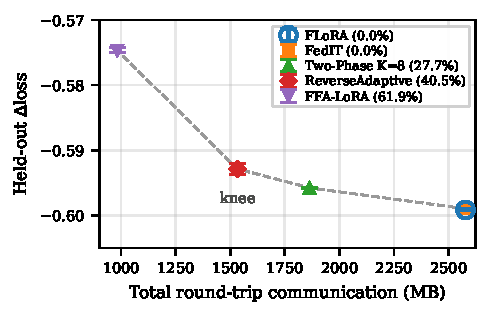
\includegraphics[width=0.75\textwidth]{Fig1.pdf}
\caption{Measured communication-quality frontier on Alpaca-3k, TinyLlama-1.1B, IID, CUDA corpus. Five protocols, three from prior work, at four distinct operating points; error bars are one sample standard deviation over three seeds, and communication is identical across seeds. Held-out $\Delta$loss is tuned minus base on the 500-example slice defined in Methods; more negative is better. FLoRA (open circle) and FedIT (filled square) coincide at lower right. The segment from ReverseAdaptive to FFA-LoRA is markedly steeper than the segment preceding it, as quantified in the Discussion}
\label{fig:frontier}
\end{figure}

Three features of Table~\ref{tab:frontier} bear on the interpretation. The two quality metrics agree on the ordering of every pair they can resolve: across the four distinct operating points the ranking is identical on final training loss and on held-out instruction-following loss. The exception is the FLoRA and FedIT pair, which shares an operating point, where FedIT is nominally better on final loss and FLoRA nominally better on held-out loss; neither difference is statistically distinguishable ($p{=}0.588$ and $p{=}0.425$). The shape of the frontier is not an artifact of the metric chosen to construct it.

ReverseAdaptive outperforms FFA-LoRA by 0.0282 on final loss and 0.0182 on held-out loss, against per-method seed standard deviations of at most 0.0016 and 0.0008 respectively. Both protocols end training with $A$ frozen and only $B$ aggregated, and they differ chiefly in whether $A$ was learned first; ReverseAdaptive also evaluates its aggregated $B$ with a frozen $A$ that differs slightly from the one its clients trained against (Methods). Learning $A$ through a FLoRA phase before freezing it produces materially better adapters than freezing $A$ at initialization, at a cost of 550 MB in this configuration.

FedIT lands on FLoRA's communication volume exactly, to the byte, and within 0.0006 on both quality metrics. It contributes no new operating point, which is the intended result: FedIT is an independently implemented full-state protocol, so its coincidence with FLoRA is evidence that the byte accounting measures the protocol rather than an implementation artifact.

Loss differences between methods are resolved across three seeds: the 0.0141 gap between FLoRA and ReverseAdaptive at $\tau{=}0.01$ is more than twenty times the per-seed standard deviation. Paired $t$-tests on final loss give $p < 10^{-3}$ for every comparison against FLoRA except FedIT, which is correctly indistinguishable. These tests have limited power at three seeds (Supplementary Note 3), so effect sizes should be read alongside the $p$-values, and no multiplicity correction is applied in Table~\ref{tab:frontier}; Supplementary Note 3 reports the complete set of paired tests on both metrics with the correction stated.

This frontier sweeps through the fixed-$K$ Two-Phase operating points: on the MPS corpus, $\tau{=}0.002$ lands on Two-Phase $K{=}8$ communication and $\tau{=}0.001$ on $K{=}10$. Because total communication is a step function of the discrete switch round, where each round of delay changes the total by 110.0\,MB, this correspondence is not backend-invariant; Supplementary Note 4 reports that both tight-$\tau$ settings fire one round earlier on CUDA. The robust claim is that the adaptive method traverses the same frontier as the fixed-$K$ family without requiring $K$ to be specified, rather than that it reproduces particular $K$ values byte for byte.

\subsection{Replication on Dolly-15k}
\label{sec:dolly}
Table~\ref{tab:dolly} repeats the three-method comparison on Databricks Dolly-15k \cite{dolly2023}, an instruction dataset with a different length distribution and a broader task mix than Alpaca. Communication is identical to the Alpaca corpus, since the protocols are dataset-independent and ReverseAdaptive fired at round 6 on every IID seed of both datasets. The quantity of interest is therefore the quality cost of switching rather than the absolute loss.

\begin{table}[tbp]
\centering
\footnotesize
\setlength{\tabcolsep}{6pt}
\caption{Dolly-15k replication. TinyLlama-1.1B, IID, CUDA corpus, three seeds, mean $\pm$ one sample standard deviation. Gap is the held-out $\Delta$loss difference against the same dataset's FLoRA baseline, which is the quantity comparable across datasets; held-out levels are not, since base-model losses differ (1.9352 on Alpaca, 2.2608 on Dolly-15k). Differences quoted in the text are computed from unrounded values and may differ from the displayed cells in the final digit. Method: FLoRA \cite{wang2024flora}. Two-Phase and ReverseAdaptive are defined in Methods. The MB column is total round-trip communication over 15 rounds}
\label{tab:dolly}
\begin{tabular}{@{}lrrrrr@{}}
\toprule
Method & MB & Final loss & Held-out $\Delta$ & Gap (Dolly) & Gap (Alpaca) \\
\midrule
FLoRA                           & 2578.13 & $1.6544 \pm 0.0021$ & $-0.5330 \pm 0.0010$ & -- & -- \\
Two-Phase $K{=}8$               & 1863.13 & $1.6643 \pm 0.0021$ & $-0.5287 \pm 0.0010$ & 0.0043 & 0.0034 \\
ReverseAdaptive ($\tau{=}0.01$) & 1533.13 & $1.6686 \pm 0.0022$ & $-0.5268 \pm 0.0005$ & 0.0061 & 0.0063 \\
\bottomrule
\end{tabular}
\end{table}

Because held-out levels depend on each dataset's base-model loss (Methods), Table~\ref{tab:dolly} reports the gap to each dataset's own FLoRA baseline. ReverseAdaptive costs 0.0063 held-out loss on Alpaca and 0.0061 on Dolly, a shift of 0.0002, or 3.0\% of the gap's own magnitude. The quality cost of the adaptive transition is stable across these two datasets.

Two-Phase $K{=}8$ costs 0.0034 on Alpaca and 0.0043 on Dolly, a shift of 25.5\%. The claim supported here is limited to ReverseAdaptive's own cost being stable, not to a property of the protocol family.

A non-IID Dolly run at $\alpha{=}0.5$ switched at round 6 on all three seeds and reached the same 1533.13 MB, matching the IID behavior on both datasets. No Dolly FLoRA baseline was run under heterogeneity, so no quality cost is reported for that configuration.

\subsection{Convergence and Switching Behavior}
\begin{figure}[tbp]
\centering
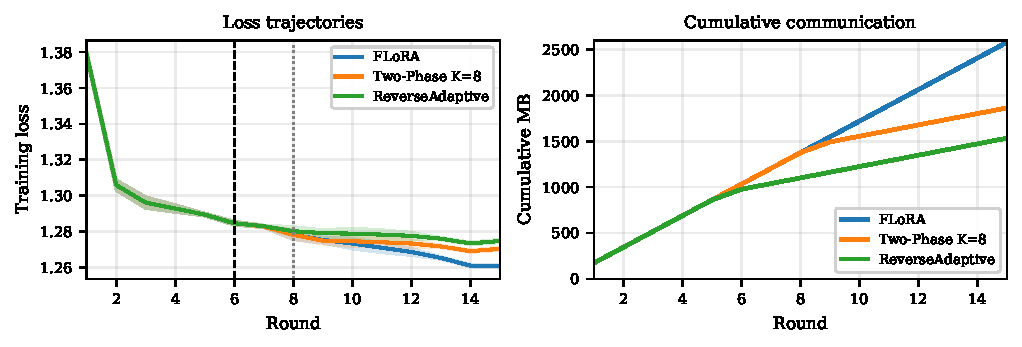
\includegraphics[width=\textwidth]{Fig2.pdf}
\caption{Left: training loss trajectories on TinyLlama-1.1B IID, MPS corpus (mean $\pm$ 1 standard deviation over three seeds). Vertical lines mark ReverseAdaptive's switch (round 6) and Two-Phase $K{=}8$'s phase boundary (round 8; the transition round, with full upload, is round 9). Right: cumulative communication on TinyLlama-1.1B (seed 42, deterministic across seeds). Slope changes mark phase transitions; look-ahead download accounting moves the broadcast slope one round before the upload slope}
\label{fig:convergence}
\label{fig:cumcomm}
\end{figure}
Fig.~\ref{fig:convergence} shows mean $\pm$ std loss trajectories (left) and cumulative communication (right) across three seeds for FLoRA, Two-Phase $K{=}8$, and ReverseAdaptive. All three methods converge similarly through the FLoRA phase. Phase transitions are visible as slight slope changes but do not destabilize training. The final ${\sim}0.01$ loss gap accumulates gradually after the switch rather than appearing as a sharp discontinuity. FLoRA stays linear at 85.94 MB per round per direction throughout. Two-Phase $K{=}8$ maintains the same slope through round 9, then reduces as B-only transmission activates. ReverseAdaptive splits off at round 6 (at TinyLlama-1.1B scale), producing the steepest savings trajectory.

The no-switch sanity baseline (ReverseAdaptive with \mbox{\texttt{switch\_threshold}}\,{=}\,{-}1.0, \mbox{\texttt{warmup\_rounds}}\,{=}\,999) produces final loss 1.2594342812 on seed 42 under the MPS corpus, matching the corresponding FLoRA run to 10 decimal places. The CUDA per-seed values in Supplementary Note 2 differ, as expected across backends; the guarantee is a within-backend statement. Upload and download match to the byte across all 15 rounds.
Disabling the switch requires a negative threshold rather than a small positive one, for reasons set out in Supplementary Note 1.

\subsection{Downstream Evaluation}
Supplementary Tables S1--S2 present downstream results on MMLU \cite{hendrycks2020measuring}, ARC-Easy \cite{clark2018arc}, BoolQ \cite{clark2019boolq}, and HellaSwag \cite{zellers2019hellaswag}. MMLU is excluded from TinyLlama-1.1B comparisons: base accuracy of 0.250 on 4-way multiple choice indicates chance-level performance, making the benchmark uninformative at 1.1B scale.

At TinyLlama-1.1B (Supplementary Table S1), all federated methods cluster within 1.0 percentage points of each other across the three informative benchmarks and regress modestly relative to the base model (Discussion).

At LLaMA-3.2-3B scale, the three federated methods are indistinguishable on downstream benchmarks within seed variation. Mean accuracies across three seeds differ by at most 0.5 percentage points on any benchmark, and the per-method error bars overlap on every benchmark. Relative to the base model they do not regress as at 1.1B (Discussion): the LLaMA base achieves MMLU 0.544, ARC-Easy 0.832, BoolQ 0.706, and HellaSwag 0.540, and every federated method matches or exceeds the first three while sitting 0.1 to 0.5 percentage points below the base on HellaSwag.

\subsection{Threshold Ablation}
\label{sec:ablation}
Supplementary Table S3 and Fig.~\ref{fig:ablation} characterize how $\tau$ controls the savings-quality tradeoff. Since $\tau$ bounds a relative rather than an absolute loss improvement, the values below are fractions of the previous round's loss: $\tau{=}0.01$ requires the loss to fall by at least 1\% in a round for the FLoRA phase to continue. The method has a sensitive regime for $\tau \leq 0.002$: at $\tau{=}0.002$ the switch occurs at round 9, matching Two-Phase $K{=}8$; at $\tau{=}0.001$ the switch occurs at round 11, matching Two-Phase $K{=}10$. For $\tau \geq 0.005$ the method saturates: the switch fires at round 6, the first round after warmup. All rows for $\tau \in \{0.005, 0.010, 0.020, 0.050, 0.100, 0.200\}$ produce identical results.

A practitioner seeking maximum savings can set $\tau$ anywhere in $[0.005, 0.2]$ without precision loss. The $\tau{=}0.001$ and $\tau{=}0.002$ operating points show the switch round responding to the loss trajectory.

\begin{figure}[tbp]
\centering
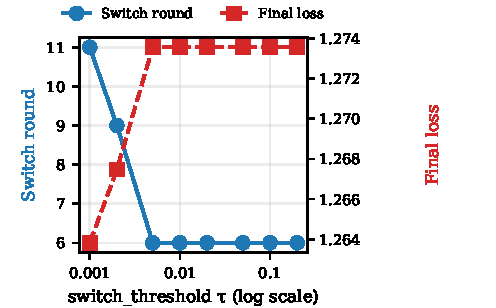
\includegraphics[width=0.75\textwidth]{Fig3.pdf}
\caption{ReverseAdaptive threshold sensitivity (TinyLlama IID, seed 42, MPS corpus). Loss values are not comparable with the CUDA results in Table~\ref{tab:frontier}, and the $\tau$=0.001 and $\tau$=0.002 settings switch one round earlier on CUDA (Supplementary Note 4)}
\label{fig:ablation}
\end{figure}

\subsection{Scale Validation}
Table~\ref{tab:llama_iid} and Fig.~\ref{fig:scale} confirm that the Pareto structure observed at TinyLlama-1.1B is preserved at LLaMA-3.2-3B.

Three random seeds (42, 123, 456) were run for each of FLoRA, Two-Phase $K{=}8$, and ReverseAdaptive. Communication for FLoRA and Two-Phase $K{=}8$ is protocol-deterministic and has no seed-to-seed variance; ReverseAdaptive's spread of $\pm 105.0$ MB reflects its switch rounds of 7, 8, and 9 across the three seeds (mean $8.0 \pm 1.0$).

\begin{table}[tbp]
\centering
\footnotesize
\setlength{\tabcolsep}{6pt}
\caption{LLaMA-3.2-3B IID results. ReverseAdaptive uses $\tau{=}0.01$. The MB column is total round-trip communication over 15 rounds and savings are against FLoRA. Mean $\pm$ 1 standard deviation across three random seeds (42, 123, 456). ReverseAdaptive switch rounds: 7, 8, 9. FLoRA and Two-Phase $K{=}8$ communication is protocol-deterministic; ReverseAdaptive communication varies with switch round}
\label{tab:llama_iid}
\begin{tabular}{@{}lrrr@{}}
\toprule
Method & Final loss & MB & Savings \\
\midrule
FLoRA & $1.3724 \pm 0.0009$ & 2625.0 & 0\% \\
Two-Phase $K{=}8$ & $1.3938 \pm 0.0011$ & 1942.5 & 26.0\% \\
ReverseAdaptive & $1.3938 \pm 0.0036$ & $1837.5 \pm 105.0$ & $30.0 \pm 4.0$\% \\
\bottomrule
\end{tabular}
\end{table}

\begin{figure}[tbp]
\centering
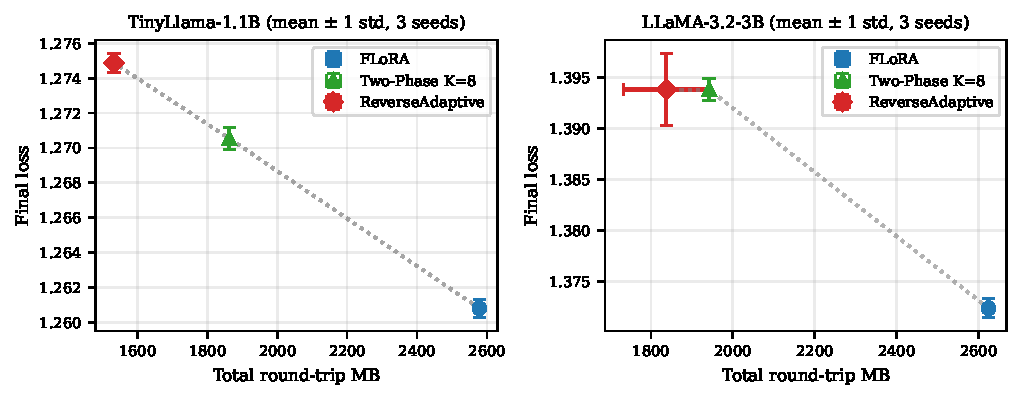
\includegraphics[width=\textwidth]{Fig4.pdf}
\caption{Scale validation. Left: TinyLlama-1.1B, CUDA corpus (mean $\pm$ 1 standard deviation over three seeds). Right: LLaMA-3.2-3B, MPS corpus (mean $\pm$ 1 standard deviation over three seeds). Both panels show the three federated methods on the same axes. Dotted polyline connects the three method points on each panel. The Pareto structure (downward slope from FLoRA to ReverseAdaptive) is preserved across scales. Y-axis ranges differ between panels because absolute training loss is model-dependent; the relative Pareto shape is the invariant being validated. ReverseAdaptive's larger error bar at LLaMA-3.2-3B reflects across-seed variance in switch round (7, 8, 9)}
\label{fig:scale}
\end{figure}

The communication savings are slightly lower at 3B than at 1.1B: 26.0\% vs.\ 27.7\% for Two-Phase $K{=}8$, and 30.0\% vs.\ 40.5\% for ReverseAdaptive. The B-only fraction of the full state is 40\% at LLaMA-3.2-3B (vs.\ 36\% for TinyLlama) due to different grouped-query attention (GQA) configurations, meaning each B-only round saves a smaller fraction of the full payload at 3B scale.

At LLaMA-3.2-3B, ReverseAdaptive and Two-Phase $K{=}8$ reach final losses differing by $1.25 \times 10^{-5}$, roughly 350 times smaller than the 0.0043 separating them at TinyLlama-1.1B. A paired $t$-test over three seeds gives $p = 0.997$ with a 95\% confidence interval of $[{-}0.0114, 0.0114]$. That interval contains the 1.1B effect size, so the test cannot distinguish no difference from a difference as large as the one observed at 1.1B, and the result is reported as a statement about effect size rather than as evidence of equivalence. ReverseAdaptive also saves 4.0 percentage points more mean communication than the fixed $K{=}8$ configuration (30.0\% against 26.0\%), because two of its three seeds switch before round 9, at rounds 7 and 8. The same threshold $\tau{=}0.01$ used at TinyLlama-1.1B produced this behavior with no scale-specific tuning.

\section{Discussion}
\label{sec:discussion}

In mobile or Internet of Things (IoT) federated settings where uplink bandwidth is scarce and metered, cutting round-trip communication by 30 to 40\% can change the economic viability of federated fine-tuning. At TinyLlama-1.1B the 40.5\% reduction costs 0.0063 in held-out instruction-following loss. Whether that trade is acceptable is a deployment decision rather than a universal one, and the frontier in Results is intended to let a practitioner make it explicitly: the same measurements show that accepting a further 21.3 points of savings costs roughly five times more quality per point. Kairouz et al. \cite{kairouz2021advances} identify communication as a fundamental open problem in federated learning at scale, and measured byte-level reporting is a prerequisite for addressing it.

\label{sec:choosing}
The Two-Phase protocol requires a practitioner to select $K$ before training begins, without knowing when the loss plateau will occur for a given model-dataset combination. This is a hyperparameter that must be tuned per dataset, per model, and potentially per client population: precisely the kind of manual configuration that slows deployment in production federated systems. ReverseAdaptive replaces it by monitoring the signal that $K$ was meant to approximate.

The criterion transfers across model scales because it is scale-free. Since $\tau$ bounds a relative loss improvement, the same numerical value encodes the same stopping condition at any absolute loss level, so it carries across models whose losses differ in magnitude; an absolute improvement threshold would not, since a fixed loss delta that plateaus one model's training would fire immediately or never on another. Using the same $\tau{=}0.01$, ReverseAdaptive fires at round 6 on TinyLlama-1.1B and at a mean of round $8.0 \pm 1.0$ on LLaMA-3.2-3B, with no scale-specific retuning. At $\tau{=}0.01$ the IID switch rounds at both scales match exactly across the MPS and CUDA backends (see Supplementary Note 4), so the cross-scale comparison does not rest on corpora that disagree about when the switch occurred.

Two details refine this result. At TinyLlama scale and $\tau{=}0.01$ the switch fires at round 6 in every MPS run across all three partition settings and in every Dolly-15k run, and round 6 is the first round after the warmup period $W{=}5$; on CUDA one $\alpha{=}0.1$ partition fires at round 7 instead, as Supplementary Note 4 reports. At $\tau{=}0.01$ and this scale the switch therefore fires as early as the warmup allows, which is the knee of the frontier; smaller thresholds move the switch along the frontier, with $\tau \leq 0.002$ yielding switch rounds of 9 and 11 (Results). Across seeds in IID training, switch round varies only at LLaMA-3.2-3B, where three runs give rounds 7, 8, and 9; those runs also differ in code revision (see below), so the variation across those three runs cannot be attributed to training dynamics alone. Two model sizes and two datasets do not establish that $\tau{=}0.01$ is a universal default; they establish that a single value carried across the two scales tested without retuning.

Where ReverseAdaptive sits on the frontier matters more than which fixed $K$ it happens to match. Moving from FLoRA to ReverseAdaptive buys 40.5 percentage points of communication savings at a held-out cost of 0.0063, or $1.56 \times 10^{-4}$ per point. Moving onward to FFA-LoRA buys a further 21.3 points at a cost of 0.0182, or $8.54 \times 10^{-4}$ per point, 5.5 times more expensive per point saved. The frontier has a knee and ReverseAdaptive sits at it. A practitioner who takes the first tranche of savings and declines the second is making the trade the measured data supports, and the value of the adaptive rule is that it locates that point without $K$ being guessed in advance.

\needspace{4\baselineskip}
\label{sec:measuredbytes}
Federated LoRA work commonly reports communication savings as parameter-count ratios \cite{zhang2024federatedgpt,sun2024ffalora,wang2024flora,bai2024flexlora}, conflating how many parameters exist with how many bytes a protocol transmits. The practice is not universal: FedSRD \cite{yan2026fedsrd} and FLoRIST \cite{ramesh2026florist} both report measured per-round communication in megabytes. Aggregate megabyte totals, however, do not separate two quantities that govern switching protocols and that a parameter ratio cannot express.

Architectural choices such as GQA fix the B-only fraction in ways a parameter ratio does not anticipate. TinyLlama-1.1B's GQA makes B-only transmission save exactly 36\% rather than the 50\% a non-GQA count suggests, and LLaMA-3.2-3B's different GQA configuration yields exactly 40\%. A theoretical 50\% savings claim made for one model family does not transfer to another without architectural accounting.

The transition round carries a cost that parameter-ratio analyses omit. At the FLoRA-to-FFA-LoRA boundary the upload is full while the broadcast is already B-only, so exactly one directional payload is upgraded from B-only to full. On TinyLlama this costs 55.0 MB, and the figure does not depend on the switch round: totals that ignore the transition would be 928.13, 1478.13, and 1808.13 MB for switch rounds 1, 6, and 9, against measured totals of 983.13, 1533.13, and 1863.13. What varies with the number of remaining rounds is the penalty's share of the total, not its size. A protocol upgrading both directions at the boundary would pay 110.0 MB; the look-ahead broadcast halves it.

Total communication across the entire corpus is one closed-form expression in one discrete parameter. For a switching protocol with switch round $s$ over $N$ rounds, uploads are full for rounds $1 \ldots s$ and broadcasts for rounds $1 \ldots s{-}1$, so $2s-1$ directional payloads are full and the total is $55(2s-1) + 928.125$ MB on TinyLlama and $52.5(2s-1) + 1050$ MB on LLaMA-3.2-3B, where $928.125$ and the non-switching endpoint $2578.125$ are exact. FFA-LoRA is $s{=}1$, ReverseAdaptive $s{=}6$, Two-Phase $K{=}8$ is $s{=}9$, and Two-Phase $K{=}10$ is $s{=}11$; every measured total reported at full ten-client participation lands on that lattice to the byte; the two reduced-participation runs in Supplementary Note 2 scale off the lattice in proportion to the active client count. The $2s-1$ arises from the harvest rule rather than from the protocol: an implementation that froze the server's existing global $A$ would upgrade no directional payload at the boundary and give $110(s-1) + 928.125$ instead. A non-switching protocol has all $2N$ directional payloads full and is not a point on the lattice: FLoRA is the separate endpoint at $55 \times 30 + 928.125 = 2578.125$ MB. The lattice spacing of 110 MB per round is also why no continuous $\tau$ reproduces a fixed-$K$ total robustly, as Results notes.

This implementation charges FFA-LoRA slightly more than its design requires. FFA-LoRA freezes $A$ at initialization, so every client's $A$ equals the shared initial value at every round and never needs transmitting. The measured 983.13 MB nonetheless includes the 55.0 MB seeding upload, because the server harvests $A$ from the first client's uploaded state rather than deriving it from the initialization (Methods). An implementation faithful to the design reaches the floor of 928.13 MB, raising FFA-LoRA's savings from 61.87\% to 64.00\%, widening the ReverseAdaptive-to-FFA-LoRA segment from 21.3 to 23.5 percentage points, and moving the marginal cost ratio from 5.5 to 5.0. The knee conclusion is unchanged. The same harvest rule governs Two-Phase and ReverseAdaptive. For Two-Phase the harvested $A$ is the round-$K$ global $A$ the server already holds, so freezing that value directly would leave training unchanged and remove the 55.0\,MB seeding upload. For ReverseAdaptive the harvested $A$ carries one epoch of local adaptation, so freezing the held global $A$ instead would change the adapter as well as the bytes, and is untested.

\label{sec:baseregression}
Federated Alpaca-3k \cite{taori2023alpaca} instruction tuning regresses TinyLlama-1.1B \cite{zhang2024tinyllama} on all three informative zero-shot benchmarks: ARC-Easy by 2.2 to 2.8 percentage points depending on method, BoolQ by 6.4 to 7.4, and HellaSwag by 2.8 uniformly. At LLaMA-3.2-3B \cite{dubey2024llama3} the same procedure is flat-to-positive on MMLU, ARC-Easy, and BoolQ and within 0.5 percentage points of the base on HellaSwag. The cross-scale contrast is consistent with a model-capacity explanation: TinyLlama-1.1B may lack the parameter budget to absorb instruction tuning without distributional drift on these benchmarks, though a single dataset and two scales cannot rule out other explanations.

The same procedure improves substantially on the objective it optimizes. On the held-out Alpaca slice the base model scores 1.9352 (perplexity 6.9254) and every fine-tuned checkpoint scores between 1.3349 and 1.3608 (perplexity 3.80 to 3.90). The regression is a divergence between the training objective and these benchmarks rather than a training failure, and it is why quality is reported here as held-out instruction-following loss. The held-out slice is drawn from the same distribution as the training data, so it measures instruction following on unseen examples and is not evidence of generalization to unrelated tasks.

The regression is independent of aggregation method. Cross-method spread at TinyLlama scale is 0.006 on ARC-Easy, 0.010 on BoolQ, and 0.000 on HellaSwag, so the zero-shot benchmarks do not separate protocols that the held-out metric separates at $p < 0.05$. These accuracies are single-seed (seed 42, MPS corpus), unlike the three-seed CUDA results in Table~\ref{tab:frontier}, so the spreads carry no variance estimate and indicate insensitivity rather than establishing equivalence.

The BoolQ result admits a specific account. The base model's accuracy of 0.626 closely matches BoolQ's natural yes-class rate of approximately 0.62, suggesting the base exploits a yes-biased prior. Instruction tuning attenuates that prior, which is why BoolQ moves furthest of the three.

\label{sec:limitations}
The experiments use two instruction-following datasets (Alpaca-3k \cite{taori2023alpaca} and Dolly-15k \cite{dolly2023}) and a single task type. Generalization to classification tasks, longer training runs, or generation-quality metrics is not characterized. Quality is measured as held-out loss on examples drawn from the same distribution as the training data, which captures instruction following on unseen examples rather than transfer to unrelated tasks.

FFA-LoRA and FedIT were evaluated on Alpaca only, so Table~\ref{tab:dolly} compares three protocols where Table~\ref{tab:frontier} compares five. The cross-dataset result therefore speaks to the cost of the adaptive transition rather than to the stability of the whole frontier across datasets.

The study covers only Llama-style decoder-only architectures with LoRA targeting \mbox{\texttt{q\_proj} and \texttt{v\_proj}}. Other architectures, encoder-decoder models, larger target sets, or heterogeneous rank configurations may produce different B-only fractions and different savings profiles. The reported percentages are specific to this target set and to the grouped-query attention configurations of the two models tested.

The simulation assumes full client participation in every round. Real federated deployments typically involve partial participation, where only a fraction of clients respond per round. The effect of partial participation on transition-round timing and on ReverseAdaptive's plateau detection is not studied here.

Non-IID partitions are constructed by Dirichlet skew over instruction-length buckets rather than over semantic labels; Alpaca carries no class labels, and Dolly-15k's category field was not used. This induces heterogeneity in task form. Heterogeneity in task semantics, which is what semantic-class partitioning models in classification settings, is untested.

No real-world network conditions are simulated. Byte counts are measured from the tensors actually transmitted, but network latency, packet loss, and bandwidth constraints are not modeled, so wall-clock communication time is not predicted.

No differential privacy (DP) analysis is included. FFA-LoRA \cite{sun2024ffalora} was originally motivated in part by DP-friendliness; the transition-round dynamics of the bidirectional B-only protocol may affect DP accounting in non-obvious ways that warrant separate study.

At the transition round the server freezes $A$ from the first client's uploaded state. For ReverseAdaptive this value differs from the $A$ against which clients train $B$ after the switch, and the effect of that mismatch on its reported quality is not measured (Methods). Freezing the global $A$ the server already holds would remove the seeding upload and is untested, so the 55.0\,MB transition cost and ReverseAdaptive's quality figures are properties of this implementation rather than of phase-switching protocols in general.

Runs were produced across more than one code revision, some including local modifications that were not committed at run time. The primary CUDA corpus spans two revisions, and the FLoRA and FedIT rows of Table~\ref{tab:frontier} sit on either side of that boundary while remaining statistically indistinguishable, which indicates that the combined algorithmic and revision difference across that boundary is roughly 0.0006 in final loss. The LLaMA-3.2-3B results are not single-revision: the three seeds were produced at three revisions, so the variability reported there combines seed and environment variation.

LLaMA-3.2-3B experiments use three random seeds with downstream evaluation per checkpoint. Seed-to-seed evaluation noise within a single checkpoint is not separately characterized. At TinyLlama-1.1B, downstream evaluation is single-seed per checkpoint while training uses three seeds.

Future work should address partial participation, non-Llama architectures, semantic heterogeneity, and real network conditions to validate deployment claims more broadly. Composing the bidirectional B-only protocol with gradient compression techniques \cite{alistarh2017qsgd,lin2017deep} for savings beyond the B-only floor is a natural extension. Per-layer adaptive phase-switching, where different transformer layers switch at different rounds based on their individual loss-plateau signals, is another direction.

\label{sec:conclusion}
In summary, byte-level measurement places five federated LoRA protocols, three from prior work, on one communication-quality frontier with a knee: savings beyond ReverseAdaptive cost roughly five times more held-out quality per point than savings up to it, and the adaptive rule locates that point without a phase boundary being specified in advance. Learning $A$ through a FLoRA phase before freezing it produces materially better adapters than freezing it at initialization. As federated deployments expand into privacy-sensitive domains, reporting what protocols actually transmit, rather than what a parameter count predicts, is a prerequisite for comparing them.

\needspace{5\baselineskip}
\section{Methods}
\label{sec:method}

\subsection{Background and notation}
Each of $N$ clients holds a local dataset. A shared base model has weight matrices $W$. LoRA \cite{hu2022lora} parameterizes updates as $\Delta W = BA$ where $B$ is $d \times r$ and $A$ is $r \times k$. In each federated round, clients train their local adapters for one epoch, upload some representation to the server, and receive a global state.

The communication cost of a round is the sum of upload bytes and download bytes. The B-only fraction of the full state is not the 50\% that counting parameters alone suggests, because grouped-query attention (GQA) fixes the ratio of $B$ to $A$ parameters; Implementation details below derives the exact fractions of 36\% for TinyLlama-1.1B and 40\% for LLaMA-3.2-3B.

\subsection{Bidirectional B-only protocol}
\textbf{Phase 1 (FLoRA, rounds 1 to $K$).}
The server runs FLoRA aggregation \cite{wang2024flora}: client states are stacked and compressed via SVD to produce a global $(A_{\text{global}}, B_{\text{global}})$. Both upload and download payloads are full state.

\textbf{Transition (round $K{+}1$).}
Clients train with $A$ frozen at the broadcast round-$K$ global value and still upload full state $(A_i, B_i)$, because the server needs the $A$ matrices to compute and cache $A_{\text{frozen}}$. The server runs FFA-LoRA \cite{sun2024ffalora} aggregation for the first time, caches $A_{\text{frozen}}$, and broadcasts only $B_{\text{global}}$; clients keep the $A$ they already hold.

\textbf{Phase 2 steady state (rounds $K{+}2$ onward).}
Clients upload only $B_i$; the server reconstructs the full state as $(A_{\text{frozen}}, B_i)$ before aggregation. The server broadcasts only $B_{\text{global}}$; clients retain $A_{\text{frozen}}$ locally.

\textbf{Look-ahead download accounting.}
This produces a one-round asymmetry: download savings begin one round before upload savings. The experiment runner records this consistently, ensuring reported totals are accurate rather than optimistic.

Supplementary Algorithm S1 specifies the server-side decision logic per round.

\subsection{ReverseAdaptive aggregator}
ReverseAdaptive replaces the fixed boundary $K$ with an adaptive loss-plateau signal. After a warmup period of $W$ rounds (default $W{=}5$), it monitors the \emph{relative} per-round loss improvement $\rho_r = (\ell_{r-1} - \ell_r) / \ell_{r-1}$. When $\rho_r < \tau$ for the first time, the aggregator switches to FFA-LoRA \cite{sun2024ffalora} mode permanently and instantaneously, with no intermediate phase. Because $\rho_r$ is a ratio of losses, $\tau$ is a dimensionless fraction rather than a loss difference, and its interpretation does not depend on the absolute scale of the loss for a given model or dataset; this scale-free construction is intended to let a single $\tau$ carry across model sizes without retuning, which Discussion examines. A complementary stability detector reverts to FLoRA if loss increases by more than 10\% after switching. No revert occurred in any ReverseAdaptive run reported in this paper, across both datasets, both model scales, all three partition settings, and the full threshold ablation.

The choice of $\tau$ trades communication savings against final training loss. Small $\tau$ delays the switch; large $\tau$ triggers it at the first eligible round after warmup. Results characterizes this tradeoff empirically.

The loss-plateau signal is chosen for its simplicity, its availability without additional instrumentation, and the fact that it tracks the quantity a practitioner optimizes. Alternative signals such as the gradient norm of $A$ or the singular value spectrum of stacked client matrices offer a different view of whether $A$ has converged and are left to future work.

Algorithm~\ref{alg:reverseadaptive} specifies the aggregator's per-round decision logic.

\begin{algorithm}[t]
\centering
\caption{ReverseAdaptive aggregator (per round)}
\label{alg:reverseadaptive}
\footnotesize
\begin{algorithmic}[1]
\Require round $r$, current loss $\ell_r$, prior loss $\ell_{r-1}$,
         warmup $W$, threshold $\tau$, current mode $m$, \texttt{client\_states}
\Ensure \texttt{global\_state}, updated mode $m$
\State $\rho_r \leftarrow (\ell_{r-1} - \ell_r) \,/\, \ell_{r-1}$ \Comment{relative improvement}
\If{$m = \text{FLoRA}$ \textbf{and} $r > W$ \textbf{and} $\rho_r < \tau$}
    \State $m \leftarrow \text{FFA-LoRA}$
    \State log event $(r, \texttt{switch\_to\_ffa})$
\ElsIf{$m = \text{FFA-LoRA}$ \textbf{and} $\ell_r > 1.1 \cdot \ell_{r-1}$} \Comment{revert}
    \State $m \leftarrow \text{FLoRA}$
    \State reset $A_{\text{frozen}}$
    \State log event $(r, \texttt{revert\_to\_flora})$
\EndIf
\If{$m = \text{FFA-LoRA}$}
    \State \Return \textsc{FFA-LoRA-Aggregate}(\texttt{client\_states})
\Else
    \State \Return \textsc{FLoRA-Aggregate}(\texttt{client\_states})
\EndIf
\end{algorithmic}
\end{algorithm}

\subsection{Implementation details}
\label{sec:implementation}
\textbf{Byte tracking.}
Per-round upload and download megabytes are recorded in \texttt{results.json}. Megabytes are reported as $2^{20}$ bytes. Byte counts use the dtype in which parameters are transmitted: float32 (4 bytes/param) for TinyLlama-1.1B and float16 (2 bytes/param) for LLaMA-3.2-3B, whose LoRA parameters are trained in float32 and cast back to the base dtype for transmission. A full TinyLlama LoRA state is 2{,}252{,}800 parameters over 22 layers, or 9{,}011{,}200 bytes per client per direction. All models are optimized using AdamW \cite{loshchilov2019decoupled}.

\textbf{Frozen-$A$ provenance.} At the transition round the server seeds $A_{\text{frozen}}$ from the first client's uploaded state rather than from an average across clients. The two switching protocols reach that round differently. Two-Phase fixes its boundary in advance, so clients train round $K{+}1$ with $A$ already frozen at the broadcast round-$K$ global value; the first client's $A$ is exactly that value, and the server and every client hold the same $A$ for the rest of training. ReverseAdaptive decides to switch only after the switch round's local training, which runs with $A$ trainable, so its $A_{\text{frozen}}$ is the preceding round's global $A$ plus one epoch of the first client's local adaptation at learning rate $10^{-4}$. The broadcast that follows carries only $B$, so clients never receive this value and train $B$ for the remaining rounds against the $A$ they hold at the end of the switch round. In the simulation, which trains clients in sequence on one shared model, that is the last client's locally adapted $A$, while the first client's $A$ enters the aggregated and evaluated adapter. The two differ by one epoch of local adaptation on different client data, and the effect of this mismatch on ReverseAdaptive's reported quality is not measured. Client ordering is fixed for the duration of a run, so the behavior is deterministic and reproducible. Averaging $A$ across clients at the transition round is an alternative left to future work.

\textbf{GQA B-fraction.}
For TinyLlama-1.1B with rank $r{=}16$ targeting $\{\texttt{q\_proj}, \texttt{v\_proj}\}$, the projections adapted in the original LoRA formulation \cite{hu2022lora}, accounting for GQA in the value projection, the B-only fraction of the full state is exactly 36\% rather than the 50\% a naive parameter count would suggest. The same fraction holds for the four-projection attention set, since \texttt{q\_proj} and \texttt{o\_proj} share a shape and \texttt{k\_proj} and \texttt{v\_proj} share a shape under GQA, but not for target sets that break that pairing, such as \texttt{q\_proj} alone or sets including multilayer perceptron (MLP) projections. LLaMA-3.2-3B's different GQA configuration yields exactly 40\%.

\textbf{Partition mechanics.}
Alpaca carries no class labels, so partitions that are not independent and identically distributed (non-IID) apply Dirichlet skew over a task-diversity proxy, and the same proxy is applied to Dolly-15k rather than its category field so that both datasets are partitioned identically: each instruction $s$ is assigned to one of ten buckets by character length, $\min(\lfloor |s| / 50 \rfloor, 9)$, and a Dirichlet distribution with concentration $\alpha \in \{0.5, 0.1\}$ is applied over those buckets. This induces heterogeneity in task form rather than task semantics; Discussion notes that semantic heterogeneity is untested.

\subsection{Experimental setup}
\label{sec:setup}
Supplementary Table S4 summarizes the experimental configuration. The corpus was executed on two hardware backends. A core of 34 runs on Apple silicon through the MPS backend, approximately 285 hours of compute, was re-executed on NVIDIA graphics processing units (GPUs), an RTX 4090 for TinyLlama-1.1B and an A100 40\,GB for LLaMA-3.2-3B; the cross-backend comparison is reported in Supplementary Note 4. The Dolly-15k replication and the FFA-LoRA and FedIT baseline runs were produced on the same rented hardware. Both TinyLlama-1.1B and LLaMA-3.2-3B experiments use three seeds for IID training.

\textbf{Baselines.} FFA-LoRA \cite{sun2024ffalora} and FedIT \cite{zhang2024federatedgpt} are reimplemented within this codebase rather than taken from the original authors' released code, which places all five protocols on one training loop and one byte-accounting path; their absolute results may differ from those of the original implementations. Following Sun et al., the FFA-LoRA implementation freezes $A$ at initialization: client-side $A$ parameters are set non-trainable before local optimization begins and are excluded from the optimizer parameter group, so clients train only $B$ from the first round. Clients transmit $B$ only, a measured 3{,}244{,}032 bytes per client per direction against 9{,}011{,}200 for full $A{+}B$ transmission. The former is $(32768 + 4096) \times 22$ parameters at 4 bytes each, exactly the B-only payload, and could not arise if $A$ were being transmitted. FedIT applies FedAvg independently to $A$ and $B$ and transmits full state in both directions, so its communication volume matches FLoRA's by construction.

\textbf{Prompt format.} Examples are rendered as \texttt{\#\#\# Instruction:} followed by the instruction text, then \texttt{\#\#\# Response:} followed by the output, truncated and padded to 256 tokens. Alpaca's optional \texttt{input} field, populated in roughly 40\% of examples, is not included in training or in evaluation. Dolly-15k differs in training: when its \texttt{context} field is non-empty, a \texttt{\#\#\# Context:} block carrying it is inserted between instruction and response, which applies to 913 of the 3000 training examples. The held-out evaluation omits that block for every example, including the 130 of 500 held-out examples that carry a context, so Dolly-15k held-out losses are measured on a format partly unseen in training. Every method is scored on the same format, so the between-method gaps on Dolly-15k are unaffected; the Dolly-15k levels are not comparable to a context-aware evaluation. Loss is computed over the full formatted sequence including prompt tokens, with padding masked to $-100$. This differs from the two-template formatting used in the original Alpaca release and shifts absolute loss values; because all methods are trained and evaluated identically, comparisons between methods are unaffected. Note that if the tokenizer aliases \texttt{pad\_token} to \texttt{eos\_token}, the end-of-sequence token is masked along with padding; this is consistent across all runs but is relevant to anyone recomputing the base-model reference values given below.

\textbf{Backend provenance.} Communication totals are protocol-deterministic given the switch round; the backends agree on every IID run at $\tau$=0.01 and differ by one switch round only near a switching boundary (Supplementary Note 4). Loss values differ across backends: Supplementary Note 4 reports cross-backend agreement within $0.01$ for IID settings, which exceeds some of the between-method differences reported in Results. Comparisons here are therefore made within a backend, and tables are labeled with their corpus. The five-method frontier (Table~\ref{tab:frontier}), the Dolly-15k replication (Table~\ref{tab:dolly}), and all statistical tests use the CUDA corpus, since the FFA-LoRA, FedIT, and Dolly runs exist only there. The threshold ablation (Results) and the LLaMA-3.2-3B results use MPS. Communication values are comparable across tables; loss values are comparable only within a backend. All 34 runs have a counterpart on the second backend, and Supplementary Note 4 reports the comparison.

\subsection{Held-out instruction-following metric}
\label{sec:heldout}
Final training loss measures fit to the federated objective, and the four zero-shot benchmarks do not discriminate between base and fine-tuned checkpoints at this scale (Discussion). Quality is therefore also reported as held-out instruction-following loss. From each dataset the 500-example slice \texttt{train[3000:3500]} is reserved, disjoint from the 3000 examples partitioned across clients, and mean token-level cross-entropy is computed under the prompt format described above. Each adapted checkpoint is scored against the unadapted base model, and the reported quantity is $\Delta\ell_{\mathrm{held}} = \ell_{\mathrm{tuned}} - \ell_{\mathrm{base}}$, so more negative values indicate better instruction following. Base-model reference values are 1.9352 (perplexity 6.9254) on Alpaca and 2.2608 (perplexity 9.5905) on Dolly-15k. Because the base values differ by dataset, held-out deltas are comparable within a dataset but not across datasets; the cross-dataset comparison in Results therefore compares between-method gaps rather than levels.

\backmatter

\section*{Data availability}
Analysis CSVs, run records, and scripts to regenerate tables and figures are available in the public repository at \url{https://github.com/jerryadamsfranklin/fedlora-protocols} and archived as release v1.0.1 at \url{https://doi.org/10.5281/zenodo.23111915}~\cite{franklin2026fedloraprotocols}. Final adapter states for the three seed-42 TinyLlama-1.1B runs evaluated in Supplementary Table S1 are included; other adapter checkpoints are not. A verification script in the repository recomputes the paper's principal quantitative claims from the released records.

\section*{Code availability}
Source code is available at \url{https://github.com/jerryadamsfranklin/fedlora-protocols} and archived at \url{https://doi.org/10.5281/zenodo.23111915}.

\bibliography{main}

\section*{Acknowledgements}
The Alpaca and Dolly-15k datasets are publicly available from their respective sources.

The author used Claude (Anthropic) for grammar and language editing of the manuscript and as a coding assistant for the released codebase. All technical content, analysis, and interpretations are the author's own. The author received no funding for this work.

\section*{Author contributions}
J.A.F. conceived the study, implemented the software, ran all experiments, analyzed the results, prepared the figures and tables, and wrote and revised the manuscript.

\section*{Competing interests}
The author declares no competing interests.

\section*{Additional information}
Supplementary Information is available for this paper. Correspondence and requests for materials should be addressed to J.A.F.

\end{document}
